\chapter{FTk}

Another aspect of the high-pileup environment of the HL-LHC is a vast increase in number of tracks per event. Existing track reconstruction hardware and software will not be able to keep up with this environment. This resulted in a proposal for the fast tracker (FTk) upgrade for ATLAS \cite{FTk}. The FTk is an FPGA-based method for performing online track reconstruction, for use in the inner detector. It would lie between the Level 1 and HLT triggers, as shown in Figure~\ref{fig:FTk_location}.

\begin{figure}[htbp]
    \centering
    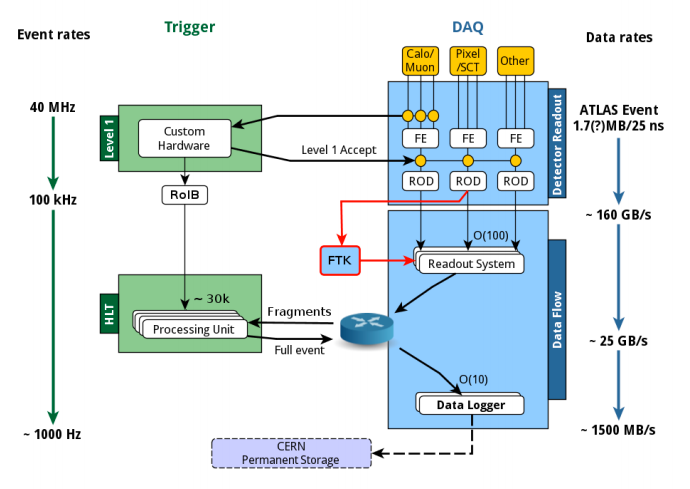
\includegraphics[width=\linewidth]{Images/Other/FTk_location.png}
    \caption{The fast tracker (FTk) lies between the Level 1 and HLT triggers.}
    \label{fig:FTk_location}
\end{figure}

I worked on the extrapolator (EXP) portion of the FTk with Professor Mark Neubaeur's team. The EXP is responsible for reconstructing 12-layer tracks (for the 12 layers of the inner detector) using preliminary 8-layer tracks and a collection of hits from the other 4 layers. A simplified layout of the FTk is shown in Figure~\ref{fig:FTk_layout}. Here we see that hits from the first 8 layers of the tracker are passed into the auxillary (AUX) board, which rapidly reconstructs candidate tracks via low-resolution pattern matching from a bank. The data formatter (DF) board sends hits from the other 4 layers to the EXP, which is then in charge of extrapolating the AUX track candidates to find matching hits on the DF layers. These hits are then used to reconstruct full tracks via the track fitter (TF), to which we then apply goodness-of-fit filtering and duplicate removal via the Hit Warrior (HW).

\begin{figure}[htbp]
    \centering
    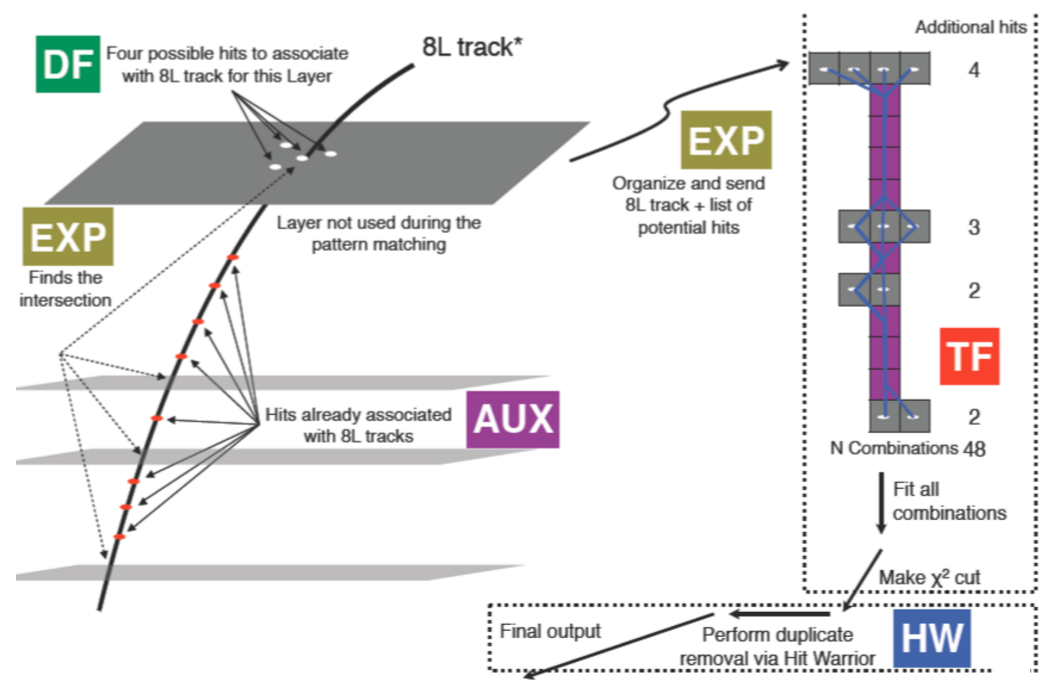
\includegraphics[width=\linewidth]{Images/Other/FTk_layout.png}
    \caption{The rough structure of the FTk.}
    \label{fig:FTk_layout}
\end{figure}

For this project, I developed a new data storage mechanism, called the HXMPP, for allowing the EXP to retrieve and organize hits. This structure was written in Verilog. It had to ensure uninterrupted data flow, being able to store and retrieve location-indexed DF hit data at 200 MHz, as well as being able to clear the memory in between events.

The logical structure of the EXP is shown in Figure~\ref{fig:EXTF}. Here, the incoming AUX info is parsed into tracks, as well as a sector ID indicating the location of the track within the detector. This info is used to retrieve matrix extrapolation constants, which are then used with the 8 AUX hits to calculate rough hit positions on the 4 DF layers. Simultaneously, the DF board sends info to the HXMPP, which is located in the bottom left corner of the diagram. The HXMPP stores the DF info, and sends it on demand when requested. Each hit is associated with a rough location, called the super-strip ID (SSID), which is used to store and retrieve the hit data. The AUX hits and matched DF hits are then passed to the track fitter for full track reconstruction.

\begin{figure}[htbp]
    \centering
    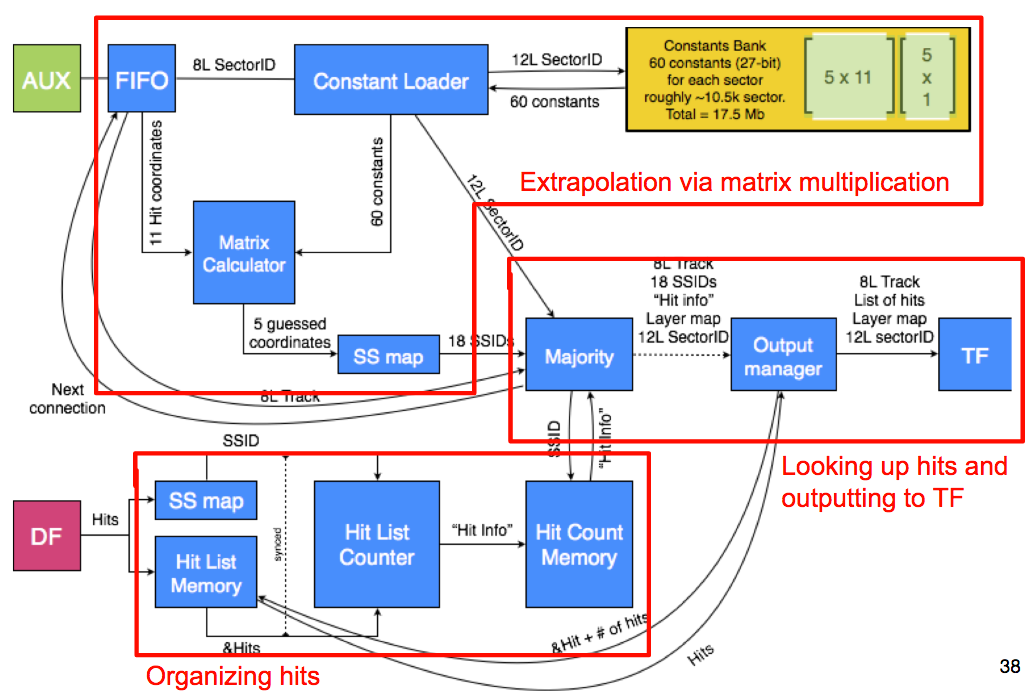
\includegraphics[width=\linewidth]{Images/Other/EXTF.png}
    \caption{The rough structure of the EXP.}
    \label{fig:EXTF}
\end{figure}

The main design objectives of the HXMPP were to be light on memory usage, and to be able to read and write new hits on every clock cycle. Reducing the memory usage was important for FPGA chip routing purposes, as having a large data storage unit in the center of the chip would make it impossible for us to hit our target processing speed. To reduce memory footprint, I implemented a new three-table structure, as shown in Figure~\ref{fig:HXMPP}.

\begin{figure}[htbp]
    \centering
    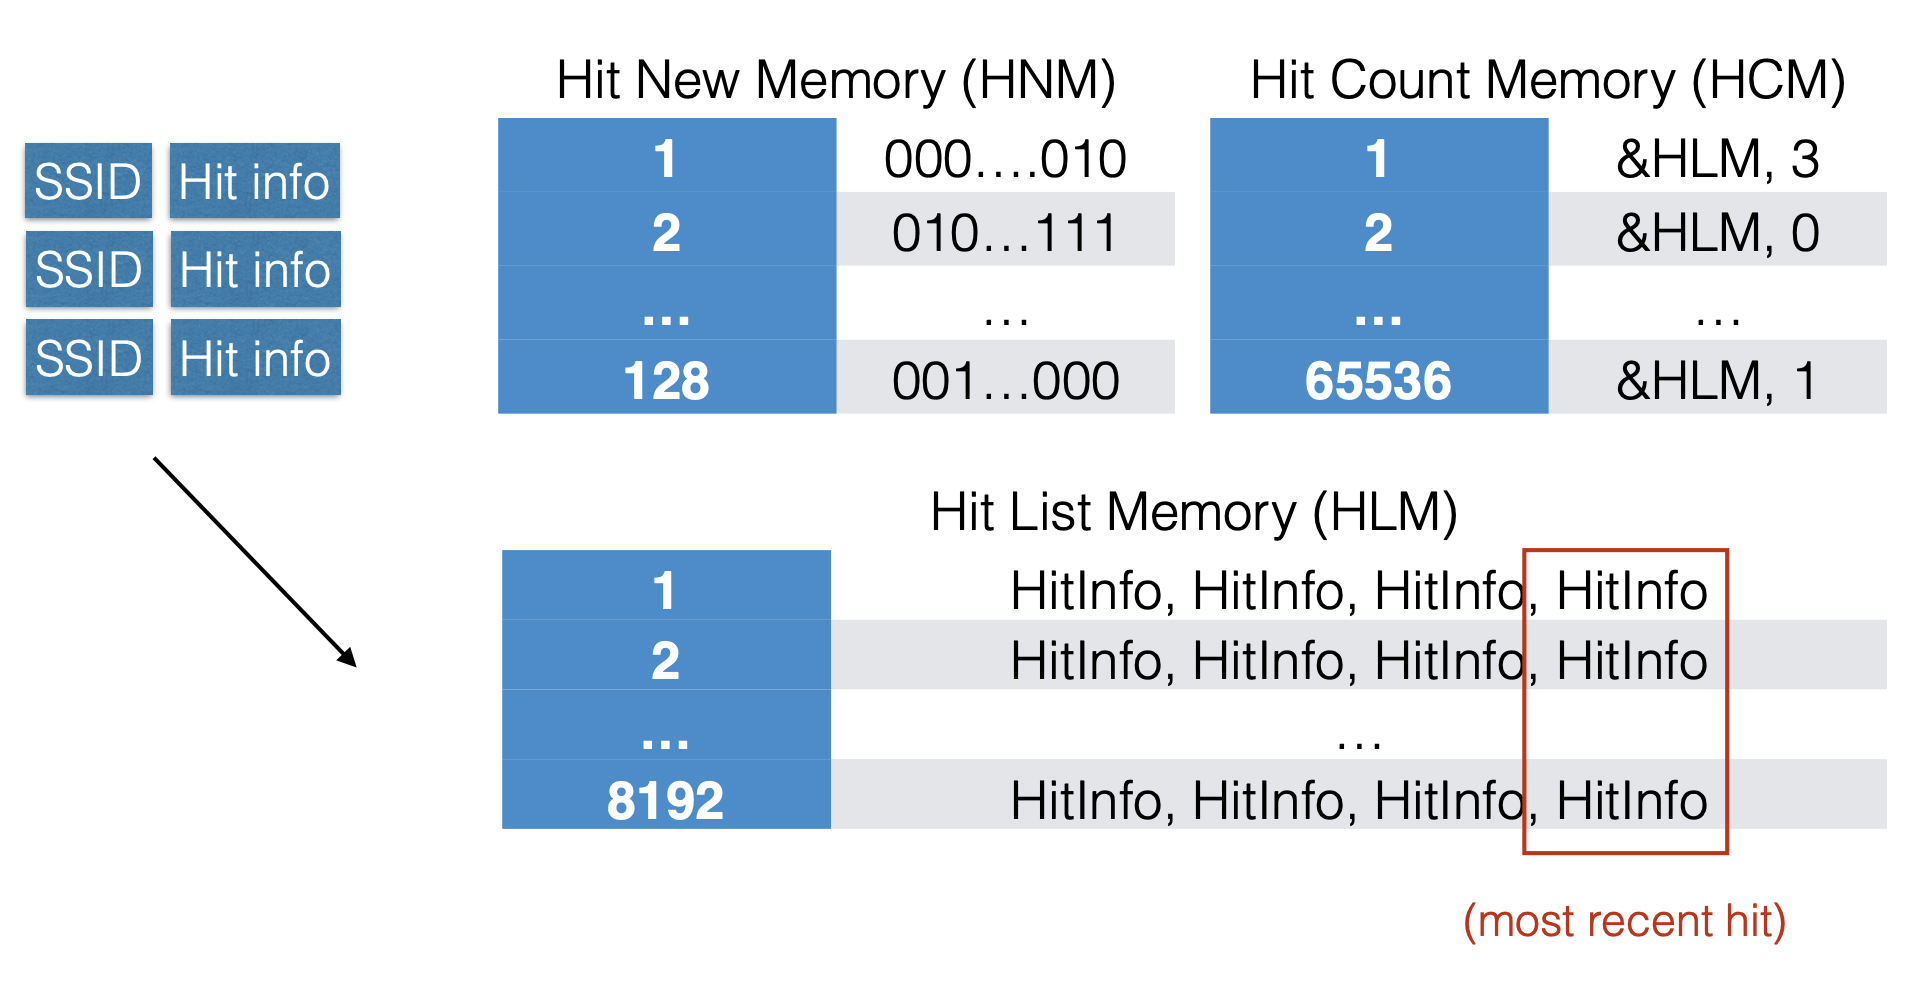
\includegraphics[width=\linewidth]{Images/Other/HXMPP.png}
    \caption{The rough structure of the HXMPP.}
    \label{fig:HXMPP}
\end{figure}

In this structure, we have a table called the hit new memory (HNM), which consists of 128 rows of 512 bits each. These bits, consisting of zeros and ones, indicate whether each SSID in the range of an EXP board has seen any new hits in the course of an event. This table is cleared in between each event, which takes 128 clock cycles. We then have a hit count memory (HCM) table with a row corresponding to each bit in the HNM, and which stores a pointer to the hit list memory (HLM) table as well as a counter indicating how many hits have been processed in that SSID during the event. The HCM and HLM can store up to 4 hits per SSID per event, and the rest are discarded. The HLM is a table with 8192 rows, with each row storing hit info for up to 4 hits.

This structure requires us to clear only the HNM between events, and only needs us to store a pointer to the next available HLM row, which is also cleared in between events. Reading from or writing to a table requires three clock cycles, and writing from each table requires a read operation first, after which the retrieved row data is updated and re-stored. Thus, in order to handle situations where multiple successive hits wish to write to the same SSID, I implemented a queuing system that allowed the HXMPP to handle simultaneous writes to a row. This system was then able to perform a read or write on every clock cycle. The code for this project is available at \url{https://github.com/BucketOfFish/HXMPP_v2}.